\section{Problema de Zunchado}
\graphicspath{{figures/}}
Se presenta un problema de zunchado de dos tubos considerados de longitud infinita. En la Figura \ref{fig:z1} se muestra la configuraci\'on inicial con interferencia y la configuraci\'on final.

\begin{figure}[!ht]
\centering
\includegraphics[width=0.7\textwidth]{zunchado1.png}
\caption{Esquema inicial y final de los tubos, luego del zunchado}
\label{fig:z1}
\end{figure}

Los datos iniciales del problema son:
\begin{itemize}
\item Material: Acero
\begin{itemize}
\item Modulo de Young: $ E=200\,\giga\pascal $
\item Coeficiente de Poisson: $ \nu=0.3 $
\end{itemize}
\item $ a=30\,\milli\metre $
\item $ b_1=35.2\,\milli\metre $
\item $ b_2=35\,\milli\metre $
\item $ c=40\,\milli\metre $
\end{itemize}

Para resolver este problema se propone:
\begin{itemize}
\item Aplicar las ecuaciones anal\'iticas
\item Resolver un modelo en Abaqus aplicando propiedades de contacto
\item Implementar un m\'etodo num\'erico con elementos finitos unidimensionales
\end{itemize}


\subsection{M\'etodo anal\'itico}
Se considera un problema de tensi\'on plana sobre la secci\'on de un tubo. Por simetr\'ia se considera que no hay variaciones en $ \theta $.

\begin{equation}
S=\binom{\sigma_r}{\sigma_\theta}
= \frac{E}{(1-\nu^2)}
\begin{pmatrix}
1 & \nu \\
\nu & 1
\end{pmatrix}
\binom{\varepsilon_r}{\varepsilon_\theta}
=D \varepsilon
\label{eq:tensionplana}
\end{equation}

A su vez podemos decir:
\begin{equation}
\varepsilon=
\binom{\varepsilon_r}{\varepsilon_\theta}=
\binom{\frac{du}{dr}}{\frac{u}{r}}
\label{eq:epsilon}
\end{equation}

En un elemento diferencial de la secci\'on se grafican las tensiones (a la izquierda) y las fuerzas resultantes (a la derecha).
\begin{figure}[h!]
\centering
\includegraphics[width=\textwidth]{zunchado2.png}
\end{figure}

Del equilibrio de fuerzas a primer orden se obtiene:
\begin{equation}
\frac{\sigma_r-\sigma_\theta}{r}+\frac{d\sigma_r}{dr}=0
\label{eq:equilibrio}
\end{equation}

Combinando (\ref{eq:tensionplana}), (\ref{eq:epsilon}) y (\ref{eq:equilibrio}) se obtiene la ecuaci\'on diferencial:
\begin{equation}
\frac{d^2u}{dr^2}+\frac{1}{r}+\frac{du}{dr}-\frac{u}{r^2}=0
\end{equation}

Cuya soluci\'on es:
\begin{equation}
u=C_1r+\frac{C_2}{r}
\end{equation}

Considerando presi\'on interna y externa, se obtiene el valor de las constantes:

\begin{equation}
C_1=\frac{(1-\nu)}{E}\frac{(a^2\,P_{in}-b^2\,P_{out})}{b^2-a^2}
\end{equation}

\begin{equation}
C_2=\frac{(1+\nu)}{E}a^2b^2\frac{(P_{in}-P_{out})}{b^2-a^2}
\end{equation}

En el problema de zunchado los tubos tienen una interferencia geom\'etrica. Para salvar esa interferencia se considera que los tubos est\'an sometidos a presi\'on (el tubo interior a presi\'on externa y viceversa). El valor de la presi\'on es aquella que cumple las relaciones:
\begin{eqnarray}
u_1=b-b_1\\
u_2=b-b_2
\end{eqnarray}
Siendo $b$ el radio final y $u_1$ y $u_2$:
\begin{eqnarray}
u_1=-P_z\left(\frac{(1-\nu)}{E}\frac{b_1^3}{b_1^2-a^2}+\frac{(1+\nu)}{E}\frac{a^2b_1}{b_1^2-a^2}\right) =-P_z\,A_1\\
u_2=P_z\left(\frac{(1-\nu)}{E}\frac{b_2^3}{c^2-b_2^2}+\frac{(1+\nu)}{E}\frac{c^2b_2}{c^2-b_2^2}\right) =P_z\,A_2\\
\end{eqnarray}

Resolviendo para $b$ se obtiene:
\begin{equation}
b=\frac{A_2\,b_1+A_1\,b_2}{A_1+A_2}=0.035112899433862\,\milli\metre
\end{equation}


La presi\'on de zunchado resulta:
\begin{equation}
P_z=8.235752182731636\cdot10^8\,\pascal
\end{equation}





\subsection{M\'etodo por contacto utilizando Abaqus}
En el entorno del programa comercial Abaqus 6.13 se modela un cuarto de la geometr\'ia del esquema de la Figura \ref{fig:z1}. Se utilizan las propiedades de contacto para forzar a las caras a tocarse. En la Figura \ref{fig:zunabaqus} se muestra una captura de pantalla de la geometr\'ia modelada. Se puede observar la condici\'on de borde para que la simetr\'ia un cuarto tenga validez.
\begin{figure}[!ht]
\centering
\includegraphics[width=0.9\textwidth]{zunabaqus.png}
\caption{Captura de pantalla de la geometr\'ia modelada en Abaqus 6.13}
\label{fig:zunabaqus}
\end{figure}
\newpage
En la Figura \ref{fig:zunab2} se grafica el campo de desplazamiento radial de los nodos. En la subsecci\'on \ref{Result1} mas resultados de este m\'etodo.
\begin{figure}[!ht]
\centering
\includegraphics[width=0.9\textwidth]{zunab2.png}
\caption{Captura de pantalla mostrando el campo de desplazamiento radial de los nodos.}
\label{fig:zunab2}
\end{figure}

La m\'axima tensi\'on de Von Mises resulta:
\begin{equation}
\sigma_{VM}=660\,\mega\pascal
\end{equation}

Esta tensi\'on es extremadamente alta. En la Tabla 1A del ASME II Parte D, el \'unico material en forma de tubo que podr\'ia servir es el SA-790 con una tensi\'on de fluencia de $\sigma_Y=650\,\mega\pascal$.


\subsection{M\'etodo por Elementos Finitos 1-D}
Se considera un problema de tensi\'on plana sobre la secci\'on de un tubo. Por simetr\'ia se considera que no hay variaciones en $ \theta $.

\begin{equation}
S=\binom{\sigma_r}{\sigma_\theta}
= \frac{E}{(1-\nu^2)}
\begin{pmatrix}
1 & \nu \\
\nu & 1
\end{pmatrix}
\binom{\epsilon_r}{\epsilon_\theta}
=D \varepsilon
\end{equation}

A su vez podemos decir:
\begin{equation}
\varepsilon=
\binom{\epsilon_r}{\epsilon_\theta}=
\binom{\frac{du}{dr}}{\frac{u}{r}}
\end{equation}

Para la discretizaci\'on del dominio se utilizan elementos anillos. Se consideran funciones de forma lineales en cada elemento unidimensional, en coordenadas locales:
\begin{equation}
N=\binom{N_1}{N_2}=\binom{\frac{1-\xi}{2}}{\frac{1+\xi}{2}}
\end{equation}

La expresi\'on del radio del elemento en la coordenada local es:
\begin{equation}
r_i=\frac{b_i+a_i}{2}+\frac{b_i-a_i}{2}\xi
\end{equation}
donde $a_i$ es el radio interno del elemento y $b_i$ el radio externo.

El jacobiano del elemento resulta:
\begin{equation}
J=\frac{dr}{d\xi}=\frac{b_i-a_i}{2}
\end{equation}

El desplazamiento en el elemento es:
\begin{equation}
u=N_1 u_1+N_2 u_2
\end{equation}

Por lo tanto la deformaci\'on de cada elemento puede expresarse:
\begin{equation}
\binom{\varepsilon_r}{\varepsilon_\theta}=
\begin{pmatrix}
\frac{dN_1}{dr} & \frac{dN_2}{dr} \\
\\
\frac{N_1}{r} & \frac{N_2}{r}
\end{pmatrix}
\binom{u_1}{u_2}=
\begin{pmatrix}
\frac{1}{J}\frac{dN_1}{d\xi} & \frac{1}{J}\frac{dN_2}{d\xi} \\
\\
\frac{N_1}{r(\xi)} & \frac{N_2}{r(\xi)}
\end{pmatrix}
\binom{u_1}{u_2}=
B\bar{u}
\end{equation}

La matriz $K$ elemental es=
\begin{equation}
K_e=\int_{a_i}^{b_i}\int_{0}^{2\pi}B^T\,D\,B\,r\,d\theta\,dr
=2\pi\,J\int_{-1}^{1}B^T\,D\,B\,r(\xi)\,d\xi
\end{equation}

Y el vector de fuerzas $f_t$ elemental resulta:
\begin{eqnarray}
f_t^e=\oint N\,P^e\,ds&=&\int_{0}^{2\pi} N\,P_{in}^e\,a_i\,d\theta- \int_{0}^{2\pi} N\,P_{out}^e\,b_i\,d\theta\nonumber\\
f_t^e&=&\pi\,a_i\,P_{in}^e\binom{1}{0}-\pi\,b_i\,P_{out}^e\binom{0}{1}
\end{eqnarray}

Como la presi\'on s\'olo se aplica en los extremos, el vector $f_t$ resulta:
\begin{equation}
f_t=
\pi
\begin{pmatrix}
a\,P_{in}\\
0\\
\vdots\\
0\\
-b\,P_{out}
\end{pmatrix}
\end{equation}
donde $a$ es el radio del borde interno y $b$ el radio del borde externo.

Finalmente, se ensambla la matriz $K$ (que resulta ser una matriz tridiagonal) y se calcula el vector $\bar{U}$ como:
\begin{equation}
\bar{U}=K^{-1}f_t
\end{equation}

\subsection{Resultados}
\label{Result1}
A continuaci\'on se muestran los resultados obtenidos comparando los tres m\'etodos, con la misma cantidad de elementos utilizados en la direcci\'on radial. Los errores relativos se calculan respecto del m\'etodo anal\'itico.

El valor de $b$ obtenido en Abaqus y en la implementaci\'on propia, para la misma cantidad de elementos, tienen asociados los siguientes errores relativos:
$$ \epsilon_b^{abaqus}=7.8864e-06 $$
$$ \epsilon_b^{propio}=7.1112e-09 $$

El error relativo en el c\'alculo de la presi\'on de zunchado para el m\'etodo propio es:
$$ \epsilon_{P_z}^{propio}=3.2567e-05$$

En la Figura \ref{fig:resS} se grafican los residuos de la tensi\'on radial en (a) y de la tensi\'on tangencial en (b).

\begin{figure}[h!]
        \begin{subfigure}[h!]{0.49\textwidth} 
	    \centering
	    \includegraphics[width=\textwidth]{figure1.pdf}
	    \caption {}
	    \end{subfigure}
        ~
        \begin{subfigure}[h!]{0.49\textwidth}
	    \centering
	    \includegraphics[width=\textwidth]{figure2.pdf}
	    \caption {}
	    \end{subfigure}
        \caption{Se grafican los residuos de las tensiones radiales (a) y tangenciales (b) comparando los m\'etodos utilizados (Abaqus e implementaci\'on propia)}
        \label{fig:resS} 
\end{figure}

Se encuentra que el error de la implementaci\'on es aproximadamente $50$ veces menor en la tensi\'on radial, y $300$ veces menor en la tensi\'on tangencial que el error de abaqus.

En la Figura \ref{fig:resU} se grafica el residuo del desplazamiento de los nodos. Se encuentra que el error utilizando la implementaci\'on propia es $700$ veces menor  que utilizando abaqus.

\begin{figure}[!ht]
\centering
\includegraphics[width=0.9\textwidth]{figure3.pdf}
\caption{Se grafica el residuo del desplazamiento.}
\label{fig:resU}
\end{figure}

A continuaci\'on se realiza un estudio de convergencia de la implementaci\'on propia. Se varia el numero de elementos y se calcula el error relativo del desplazamiento en el punto $r=b_1$ del tubo interior. En la Figura \ref{fig:eN} se grafica este residuo en funci\'on de la cantidad de elementos utilizados.

\begin{figure}[!ht]
\centering
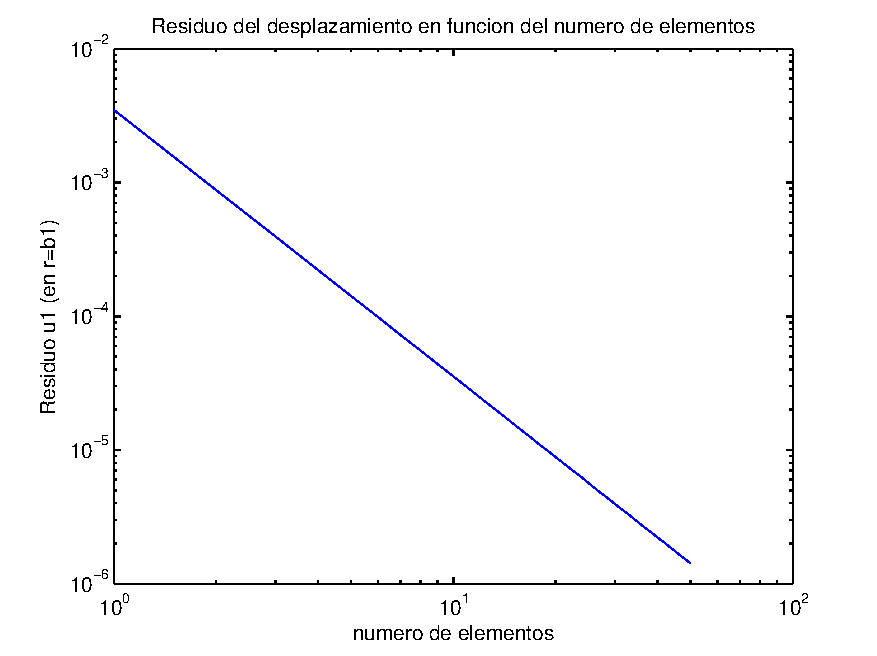
\includegraphics[width=0.9\textwidth]{figure4.pdf}
\caption{Residuo del desplazamiento del nodo $r=b_1$ del tubo interior en funci\'on del numero de elementos de la discretizaci\'on}
\label{fig:eN}
\end{figure}

Se realiza una estimaci\'on lineal sobre el gr\'afico log-log de la Figura \ref{fig:eN} resultando el residuo:
\begin{equation}
\epsilon\propto h^{1.9978}
\end{equation}